\chapter{Implementación}
Como parte del desarrollo formal del proyecto se dan a elegir distintas opciones entre dispositivos para la captación de la señal proveniente del cuerpo humano, esto es claramente notable que se elige de una gama que va desde Raspberry Pi, Arduino, Pic´s (Familia 18F), módulos de E/S basados en sensor (de National Instruments), etc.\newline

Por ello debemos poner énfasis en el dispositivo correcto, en este caso se utilizará Pic de la familia 18F, debido a que tienen un buen procesamiento de datos, entrada analógica y convertidor A/D, junto con un lenguaje de programación manejable para el tipo de función que vamos a desempeñar.\newline
\begin{floatingfigure}[r]{3cm}
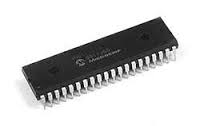
\includegraphics{imag/pic.jpg}
%\captionof{Figura}{Un poliedro}
\end{floatingfigure}


Aunque podemos utilizar los dispositivos antes mencionados, el tratamiento es el mismo únicamente se modifica la forma de atacar dichos datos y la salida respectiva, aunque no se descarta las funcionalidades que se tienen, en cierto modo se busca que este dispositivo sea practico y que pueda ser fácilmente utilizado, en este caso una persona que no dispone de los conocimientos previos para el manejo de Arduino o Raspberry evidentemente no aprovechara los recursos a comparación de un dispositivo que únicamente tenga como fin el de ser un EGC.\newpage

En términos simples toda señal (para proyectos de este tipo) recibida debe pasar por un tratamiento para poder apreciarla correctamente por el usuario final, se proponen una etapa de filtros y de acondicionamiento para que el proceso sea correcto, entre los que destacan se encuentran los que se muestran en las Figuras \ref{filtros} y \ref{filtros2}.

\begin{figure}[H]
\centering
\subfigure[A]{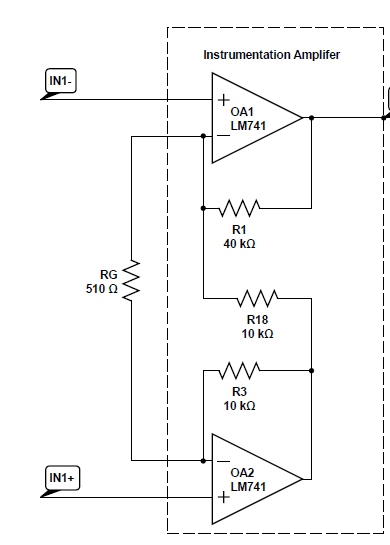
\includegraphics[scale=0.5]{imag/instrum.PNG}}
\subfigure[B]{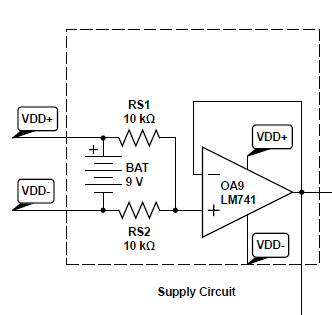
\includegraphics[scale=0.5]{imag/suply.PNG}}
\subfigure[C]{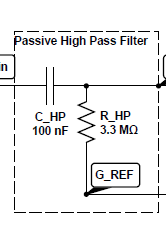
\includegraphics[scale=0.5]{imag/passive.PNG}}
\subfigure[D]{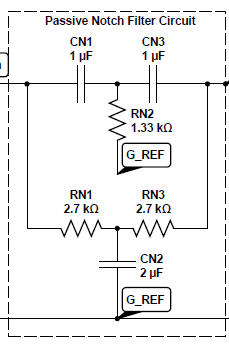
\includegraphics[scale=0.5]{imag/passive_notch.PNG}}
\caption{Filtros}
\label{filtros}
\end{figure}

\begin{figure}[H]
\centering
\subfigure[E]{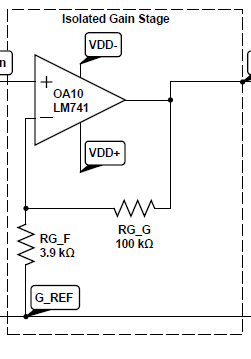
\includegraphics[scale=0.5]{imag/isolated_gain.PNG}}
\subfigure[F]{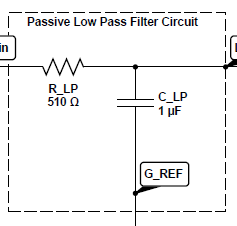
\includegraphics[scale=0.5]{imag/passive_low.PNG}}
\subfigure[G]{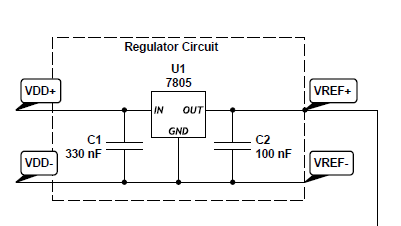
\includegraphics[scale=0.5]{imag/regulator.PNG}}
\subfigure[H]{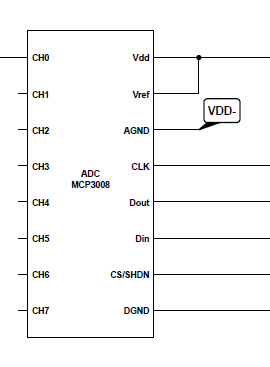
\includegraphics[scale=0.5]{imag/ADC.PNG}}
\caption{Filtros 2}
\label{filtros2}
\end{figure}
Donde cada parte se define como:
\begin{itemize}
\item[[A]] Amplificador de instrumentación.
\item[[B]] Circuito de suministro de poder.
\item[[C]] Filtro pasa-altas.
\item[[D]] Filtro pasivo notch.
\item[[E]] Etapa de ganancia.
\item[[F]] Filtro pasa-bajas.
\item[[G]] Circuito regulador.
\item[[H]] Convertidor A/D.
\end{itemize}
Estas etapas son en su mayoría recomendaciones de otros trabajos para poder realizar un proceso adecuado en la señal, aunque se consiguiera evitar alguna etapa se espera que se incluyan todas ya que esto seria optimo para un proceso integral y que no se pierda información o se le añada ruido.
\begin{figure}[H]
   	\centering
		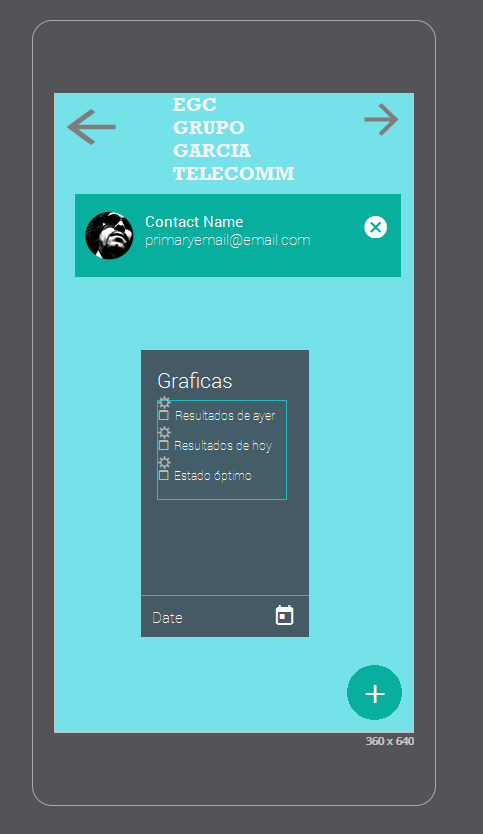
\includegraphics[width=6cm]{imag/app.PNG}
		\caption{Maquetación de la App en Android.}
		\label{app}
\end{figure}
La Figura \ref{app} es un ejemplo de como podría quedar la ventana de la aplicación esto se puede modificar fácilmente gracias a Android Studio y el software \textit{Justinmind} en este caso trabajamos con la \textit{Version (Ver. 7.5.0)}\newpage

Para la parte de interconexión entre elementos podemos utilizar un modulo embebido wifi como el que se muestra en la Figura \ref{wifi}, debemos tener en cuenta que el PIC de la familia 18F debe tener pines de TX y RX para poder enviar y recibir estas señales.
\begin{figure}[H]
   	\centering
		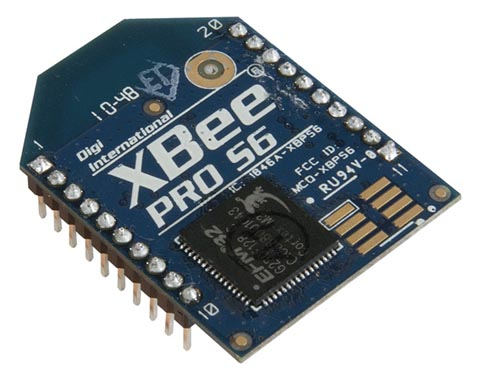
\includegraphics[width=6cm]{imag/wifi.jpg}
		\caption{Modulo embebido Wi-Fi.}
		\label{wifi}
\end{figure}

En este caso podemos utilizar el \textit{módulo embebido XBee de Digi International}, este que ofrece conectividad de serie a IEEE 802.11 (Wi-Fi).\newline

Este modulo responde a los requerimientos de bajo coste y mínimo consumo de redes inalámbricas con infraestructura 802.11, crea nuevas oportunidades en gestión de energía, automatización de procesos y factorías, sistemas de sensores, control inteligente de bienes y mercancías y otros muchos entornos, con lo cual es una buena elección de interconexión.



